\documentclass[12pt,letterpaper]{article}

%%%% NC: FOR CLARITY - can you make the bits that are just copied from the text italic? Sometimes it jumps quickly between a comment to a piece of text. Italics will help make it clearer.%%%%

%Packages
\usepackage{pdflscape}
\usepackage{fixltx2e}
\usepackage{textcomp}
\usepackage{fullpage}
\usepackage{float}
\usepackage{latexsym}
\usepackage{url}
\usepackage{epsfig}
\usepackage{graphicx}
\usepackage{amssymb}
\usepackage{amsmath}
\usepackage{bm}
\usepackage{array}
\usepackage[version=3]{mhchem}
\usepackage{ifthen}
\usepackage{caption}
\usepackage{hyperref}
\usepackage{amsthm}
\usepackage{amstext}
\usepackage{enumerate}
\usepackage[osf]{mathpazo}
\usepackage{dcolumn}
\usepackage{lineno}
\usepackage{color}
\usepackage[usenames,dvipsnames]{xcolor}
\pagenumbering{arabic}

%Pagination style and stuff
%\linespread{2} 
% NC: Cover letters don't need to be double spaced and by removing this we reduce the page count substantially! i.e. to non "losing the will to live" lengths...

=======
%\linespread{2}
\raggedright
\setlength{\parindent}{0.5in}
\setcounter{secnumdepth}{0} 
\renewcommand{\section}[1]{%
\bigskip
\begin{center}
\begin{Large}
\normalfont\scshape #1
\medskip
\end{Large}
\end{center}}
\renewcommand{\subsection}[1]{%
\bigskip
\begin{center}
\begin{large}
\normalfont\itshape #1
\end{large}
\end{center}}
\renewcommand{\subsubsection}[1]{%
\vspace{2ex}
\noindent
\textit{#1.}---}
\renewcommand{\tableofcontents}{}

\setlength\parindent{0pt}

\begin{document}

% NC: Probably want to change figure to Figure, table to Table, appendix to Appendix to be consistent.

\textbf{RE: MPE-15-254}\\
\bigskip
Dear Dr D\'{a}valos,\\
\bigskip
We are very grateful to both referees for their helpful and constructive comments, which we believe have helped us to significantly improve our paper. We have taken all of their comments on board, and respond to their points below. For improving clarity in this document, we sorted the reviewers comments as follows:
\begin{enumerate}
\item \textbf{Reviewer 1:} containing reviewer 1's major comments
\item \textbf{Reviewer 1 specific comments:} containing reviewer 1's specific comments
\item \textbf{Reviewer 2:} containing reviewer 2's comments
\end{enumerate}
Also, we uploaded two versions of the revised manuscript. Both have the exact same content but one has all the changes and additions to the main text highlighted in yellow to help with reviewing.

\section{Reviewer 1:}

\begin{enumerate}
% -----------------
% Comment 1
% -----------------
\item{\textcolor{blue}{\textbf{Novelty:} The novelty of this study should be spelled out more clearly by more a more thorough review of the literature, not just by referring to a few relevant works, but by pointing out what is so new about this study.
The authors assert that this is the first study to examine the effects of missing morphological data from a total evidence dataset, but that is what Pattinson et al. 2014 did (as well as Wiens 2005).
This study examines it in a different way with a study design that is unique and adds to the field. For example, one feature of this study that is unique is that a tree with fossils is simulated and the data simulated on that tree.
In other studies of missing data, data were removed from living taxa to determine if their positions could still be inferred (Pattinson et al. 2015; Wiens and Tiu 2012).
This study will have bearing on an old assertion that including fossils specifically may help alleviate long-branch attraction, not only additional taxa with varying amounts of missing data, as suggested by others (e.g., Wiens 2005).
Similarly, in the discussion, the authors need to point out how their results fit in with the results of previous research more clearly. }}

We thank the reviewer for this helpful comment and emphasize the novelty of this paper through the introduction, the discussion and the conclusion.
Please see specific changes outlined at reviewer 1 comments 4, 10 and 11 below.

% -----------------
% Comment 2
% -----------------
\item{\textcolor{blue}{\textbf{Graphical abstract:} Current graphical abstract does not capture the content of the article for readers in a single glance.
The authors should not use red and green together.
Figure 5 illustrates topology distance with different inference methods and varying proportions of missing data in rows vs columns and would make a better graphical abstract.
For the graphical abstract, Fig 5 needs to be made clearer in one glance what is going on.
More details are given in the comments on that figure below.}}

We gladly followed reviewer 1's graphical abstract suggestions and have changed it to be similar to Figure 5.

% -----------------
% Comment 3
% -----------------
\item{\textcolor{blue}{\textbf{Highlights:} wording seems awkward}}

We rephrased the highlights as follows: 

\begin{enumerate}[(1)]
\item The Total Evidence method places living and fossil taxa on the same phylogeny.
\item Here we test the effect of missing morphological data on Total Evidence topologies.
\item The number of living taxa with morphological data has greatest effects on topology.
\item Bayesian inference outperforms Maximum Likelihood for correct clade recovery.
\item We recommend increased sampling effort for morphological data of living taxa.
\end{enumerate}

% -----------------
% Comment 4
% -----------------
\item{\textcolor{blue}{\textbf{Introduction:} Needs stronger emphasis on what specifically is unique about this study compared to what the many other studies on missing data have done and found.
Clearly outlining the questions in this study that are left open from previous research is important because some of the findings in this study suggest that there may be more error associated with missing data than previous research has suggested.}}

We have increased our emphasis on novelty throughout the introduction by more clearly stating the difference between the present study and the literature and more clearly outlining the question of this study, as follows:

% 0(before this section)-Missing data can be a problem
% 1-And until now, not many studies

% NC: Line numbers?
Until now, few attempts have been made to study the impact of this missing data issue on phylogenetic inference in a Total Evidence framework (i.e. using both molecular and morphological data; e.g. Wiens et al., 2005; Manos et al., 2007; Pattinson et al., 2014).
% 2-These studies have done X and Y to see if missing data's a problem
These studies have assessed the effect of missing data on topology by either (1) comparing a dataset with missing data to subsets without missing data (Wiens et al. 2005); or (2) removing both molecular and some morphological data from living taxa to create artificial fossils (Manos et al., 2007; Pattinson et al., 2014).
% 3-They show that it's not a problem
Both approaches have shown that missing data are not a major problem and should not be an obstacle to combining both living and fossil species in the same phylogenies.
% 4-But they've done it a certain way
However, these studies were limited by their empirical-only approach and the use of only living taxa (Wiens et al., 2005) or the scheme of generating missing data (i.e. using the patterns from the fossil record; Manos et al., 2007; Pattinson et al., 2014).
% NC: This is still a problem (it's ok up to 4). WHY is an empirical-only approach limiting? WHY is it limiting to generate missing data using fossil patterns? 
Besides, the studies using fossil data, mainly focus on the palaeontological aspect of the question (i.e. the effect of missing data in fossils in Total Evidence matrices; Manos et al., 2007; Pattinson et al. 2014).
% NC: I don't like all these i.e.s here. Why not be specific in the text rather than throwing everything into brackets? If you're only citing manos and patterson then just say what they did.
% (next §)5-We're doing it this way

[lines 99-103 @@@] In this study, we propose a theoretical assessment of the effect of missing data in the Total Evidence method by removing living or fossil data, or all data for certain characters.
% NC: Could be more specific here and have a sentence that says. "This is an advance on previous studies because..."
We test the effect of missing data by measuring two crucial aspects of topology in both Maximum Likelihood and Bayesian phylogenies: (i) the conservation of clades and (ii) the displacement of wild-card taxa. 
% NC: Again how is this an advance. I guess it's related to this sentence from below:
% (cf. Wiens et al., 2005; Pattinson et al., 2014 measuring respectively only the clades support or the number of shared clades).


% TG: I actually rewrote this bit as well:
% NC: line numbers?
We remove data from a Total Evidence matrix by changing the values of these three parameters and then assess how this affects the resulting tree topology.
We inferred the topology from the matrices using both Maximum Likelihood and Bayesian Inference methods and measured the differences in topology using two different topological distance metrics as proxies for clade conservation (based on the Robinson-Foulds distance; Robinson and Foulds, 1981) and for wild-card taxa placement (based on the Triplets distance; Critchlow et al., 1996).
Thus, in the present study, we propose a new approach to the missing-data question, focusing on both palaeontological and neontological data (rather than just palaeontological data), using only simulated data and measuring the effects of missing data on two aspects of topology (cf. Wiens et al., 2005; Pattinson et al., 2014 measuring respectively only the clades support or the number of shared clades).
% NC: This paragraph seems to be repeating what you've already said above but in slightly more detail. Might make more sense to combine this paragraph and the one above it?

% -----------------
% Comment 5
% -----------------
\item{\textcolor{blue}{\textbf{Abbreviation:} One suggestion is to consider abbreviating Maximum Likelihood and Bayesian Inference as ML and BI respectively early in the methods and use throughout.}}

We understand the reviewer's concern.
Nonetheless, we would prefer not abbreviate these terms. 
Although they might make sentences where Maximum Likelihood and/or Bayesian Inference are stated more concise, we think spelling out the terms makes our paper clearer and does not ask the reader to look back for the actual meaning of the abbreviation (Berlin 2013; Radiology; \url{http://pubs.rsna.org/doi/abs/10.1148/radiol.12121776}).
Additionally this could lead to a confusion between ML (Maximum Likelihood) and $M_L$ (Proportion of living taxa with no morphological data).
However, we can change this at a later stage if necessary.


% -----------------
% Comment 6
% -----------------
\item{\textcolor{blue}{\textbf{Methodology - True tree:} I suggest it warrants comparing at least the 'best' tree to the 'true' tree.}}

We have now compared both the ``best'' tree and the ``missing-data'' trees to the ``true'' tree as suggested by both reviewers.
The results are available in appendix B; figure B1 and appendix C; figures C6 and C7.
The ability to recover the ``true'' tree is poor for both methods and using both metrics (Maximum Likelihood 50\% CI between approximately 0.2 and 0.3 Normalised Robinson-Foulds and Triplets metric; Bayesian consensus tree 50\% CI between approximately 0.3 and 0.4 Normalised Robinson-Foulds metric and between 0 and 0.2 Normalised Triplets metric). % NC: What are these results comparing? All missing data trees  to the true tree? True trees to best trees? Clarify.
This may be related to the size of our matrices or to the ability of the algorithms to generate the ``complete matrix'' but also to our decision to put our minimum median bootstrap acceptance at 50 rather than higher values (line @@@ in the former manuscript and @@@ in our revision).
When comparing the ``true'' tree to the ``missing data'' trees, the results are \textit{scaled down} due to the low scores of the ``true'' \textit{vs.} ``best'' trees scores.
However, we can observe the same patterns between the methods as when using the ``best'' tree (i.e. Bayesian always outperforms ML in clade conservation but does poorly in wild-card taxa placement).
An interesting feature is that the Normalised Robinson-Foulds metric actually \textit{increases} with missing data % NC: specify what is being compared, e.g. "when we compare the missing data trees to the ``true'' trees."" 
This is because the difference between the ``best'' and the ``true'' tree is high, making trees with more data more different than those with lots of missing data.
When data are missing, however, more clades are unresolved and thus closer to clades from the ``true'' trees.

Although though we agree with the comments of both reviewers that knowing the difference between the true and best/missing-data trees is important, we do not think that these results warrant inclusion in the main text.
In these simulations, we had to make a choice between (1) simulating larger matrices but with fewer chains (i.e. less variance) or (2) smaller matrices with more variance.
We deliberately made the second choice because our main question was "what is the effect of our parameters on recovering topology".
To answer this question, we maintain that comparing the best tree to the missing-data trees is the best approach for two reasons:
\begin{enumerate}
\item{The true tree is always unknown:} as we state in the manuscript: "In real world situations, the ``true'' tree is never available" (line 242 in the first manuscript and @@@ in the revision).
\item{The true tree is just the starting point of the simulations:} we use the true tree only as a starting point for our simulations.
Once generated, the true tree is fed to a cascade of algorithms and software (i.e. seqGen\{phyclust\}, rTraitDisc\{ape\}, RAxML, MrBayes) described in section 2.1 and 2.3 to get the best tree and the missing-data trees.
Comparing the latter to the true tree will answer our question "what is the effect of our missing-data parameters and the cascade of algorithms and software on recovering the true topology?".
\end{enumerate}
Therefore we added a second justification to the main text (see below this response) and added these analysis (true vs. best/missing-data trees) to the supplementary for readers that might be interested by this specific problem.

We added the following sentence to the main text to clarify and link to the supplementary analysis:

"We compare ``best'' trees to ``missing data'' trees but could also compare ``true'' trees to the ``missing data'' trees.
In practice, the difference between the ``best'' trees and the ``missing data'' trees represents the effect of our missing data parameters and of the phylogenetic methods used to infer the ``missing data'' trees.
The difference between the ``true'' and the ``missing data'' trees, however, represents the effect of our parameters used to generate the ``true'' tree and the algorithms used to generate the ``complete'' matrix as well as the effect of our missing data parameters and the phylogenetic methods used.
Because the main aim of this study is to look at the effect our missing data parameters on topological recovery, we chose to represent only the comparisons between the ``best'' trees and ``missing data'' trees.
The results of the comparisons of the ``true'' and the ``missing data'' tree are available in appendix B.
Note that this makes little difference to our overall results." line 276-280 @@@.

See also appendix B section "Differences between the ``true'' and the ``best'' trees." and reviewer 2's comment 1 below.


% -----------------
% Comment 7
% -----------------
\item{\textcolor{blue}{\textbf{Methodology - Starting tree:} The authors should at least include some analysis in which no starting tree is given, the max. likelihood 'best' tree is given, and / or the 'best' tree is given but with some perturbation.
I fear that one of the main results may be biased due to this one methodological detail - a strong prior on tree topology.
The justification given was 'to speed up the Bayesian analysis' which does not seem adequate, given these datasets are small.}}


We took on board this comment and agree with the reviewer that if using the ``true'' tree as a starting tree had an effect it would bias our results.
We therefore ran an extra analysis to test if that was the case and found that it had no major effect of the inferred tree topologies.
We performed this extra analysis on a subset of five trees with the three missing data parameters at 0\%, 10\%, 25\%, 50\% and 75\% for 20 chains. 
We compared the topology of these trees in Bayesian inference when using the ``true'' tree as a starting tree or without using a starting tree (i.e. using the default in MrBayes which is to use a different random tree for each MCMC chain).
We found no significant difference in topologies between the Bayesian inferences starting with the true tree or a random tree.
Therefore, we do not believe our results are merely the result of using a specific starting tree topology.
These results are available in the supplementary materials Appendix A (Figure A2 and Table A1) and we also added a note to the manuscript:

"We used a fixed starting tree rather than a random starting tree (default MrBayes; Ronquist et al., 2012b) to speed up our Bayesian inferences.
Note that a starting tree is not a Bayesian prior on topology \textit{per se} and using a fixed starting tree did not significantly affect topology compared to using random starting trees (see Appendix A, section ``Effect of the starting tree on Bayesian inference'')." line 323-327 @@@.
See also Appendix A section "Effect of the starting tree on Bayesian inference".


% -----------------
% Comment 8
% -----------------
\item{\textcolor{blue}{\textbf{Results - Bhattacharyya meaning:} Some descriptive statistics are given, but it would help to tell us if these differences are meaningful.
For example, on line 414 the Bhattacharrya Coefficients are given suggesting RF distances are lower for ML than BI trees at 0.69, 0.48, and 0.66 - but if this coefficient represents the probability of overlap between distributions then shouldn't the coefficients be $<$0.05 to say that one is lower than the other?
In the table, mean and median values of $<$0.01 and $>$0.85 are highlighted as being the most extreme.
Later the focus on Bhattacharyya Coefficients is 1 when distributions overlap completely and 0 when they do not - should this be the criterion?
Just make it clear early on so the readers knows what to think when they see these numbers. }}

We clarified the interpretation of the Bhattacharyya Coefficient throughout the manuscript.
We say that two distributions are significantly different when their probability of overlapping (the Bhattacharyya Coefficient) is $>$0.05 and that they are significantly similar when this probability is $>$0.95.
Even though other values (e.g. 0.85) are not conclusive, we still reported them to show the relative overlap of the distributions (i.e. two distributions with a coefficient of 0.85 are not significantly similar but are closer to each other than two distributions with a coefficient of 0.15; which are themselves not significantly different but still less close to each other than the previous ones).
We added the following statement to the main text and to the appendix B:

"The Bhattacharyya Coefficient is the probability of overlap between two distributions bounded between 0 (no overlap) and 1 (full overlap; Bhattacharyya, 1943, see Appendix B for calculation details)." lines @@@

"When the Bhattacharyya Coefficient between two distributions is $<$0.05, the distributions are significantly different.
When this coefficient is $>$0.95, the distributions are significantly similar.
Values between these two thresholds show the probability of overlap between the distributions but do not allow us to define the significance of the similarity or differences between distributions." line 419-424 @@@.

% -----------------
% Comment 9
% -----------------
\item{\textcolor{blue}{\textbf{Results - Bayesian consensus vs. Bayesian posterior:} One major finding that was not fully addressed was that the distances between the BI posterior distributions of trees do not overlap the BI best or consensus trees.
It seems from the tables in Appendix C that the topology distance metrics for Bayesian posterior distribution are similar to those for the Bayesian consensus, albeit usually lower for RF distance than the Tr distance.
In Figure 4, it seems like the distributions of metrics based on CIs for Bayesian consensus and posterior overlap up until >25\% missing data.
How then in comparisons of the distributions are they always so low (Table 1 max prob. of overlapping distributions = 0.11)?}}

The difference between the Bayesian consensus and the Bayesian posterior trees can be due to two factors:
\begin{enumerate}[I]
\item the way we assess topological recovery is slightly different in each case: for the Bayesian consensus trees, we simply compared the missing-data consensus tree to the best consensus tree; for the Bayesian posterior trees however, we randomly compared 1000 missing-data Bayesian posterior trees to 1000 best Bayesian posterior trees.
Therefore, even if the comparison methodology is the same, the fact that the second methods draws random trees means we expect the topological recovery score to be blurred in comparison to other comparisons that do not involve random comparisons.
\item the Bayesian posterior trees are always resolved and thus, in the same way as the Maximum Likelihood tree, more likely to contain false-positive nodes. On the other hand, because the consensus tree is a strict majority consensus rule, only nodes with a a good support will be represented in the tree and all other nodes will be collapsed. This reduces the number of false-positive nodes (since an unresolved tree is always better than a wrongly resolved one) and increases clade conservation but also increases the displacement of wild-card taxa (since it is likely that some Triplets will just not exist in a poorly-resolved consensus tree).
\end{enumerate}
Both points were discussed in the original manuscript lines 566-573 (or lines 645-652 @@@ in the revised version).
We expanded the paragraph to:

"Additionally, the Bayesian posterior trees performed more poorly than the Bayesian consensus tree (figure 4, table 1 and appendix C figure C5 and tables C5, C6 and C7).
This may be because the Bayesian posterior trees are always resolved and thus more likely to contain incorrectly resolved nodes (i.e. decreasing the Normalised Robinson-Foulds metric).
Conversely, the Bayesian consensus tree might not resolve nodes that are poorly supported and thus is more likely to contain only correctly resolved nodes (i.e. increasing the Normalised Robinson-Foulds metric)." lines 652-658. @@@

Concerning the last question of this comment: "How then in comparisons of the distributions are they always so low (Table 1 max prob. of overlapping distributions = 0.11)?", we apologise for the confusion here and assume it is due to our mislabeling of the figure 4 (see reviewer 1's comment 12).
In fact, when looking at all parameters separately (figure 4), there is no clear overlap between the Bayesian consensus trees and the Bayesian posterior trees (median Bhattacharyya Coefficient of 0.01; Table 1).
The maximum observed Bhattacharyya Coefficient (0.11; Table 1) is probably due to the combination of parameters: when all the parameters have many missing data, the probability of overlap between trees was slightly higher (0.11) but still really low.
For the Normalised Triplets distance however, the overlap is higher (median Bhattacharyya Coefficient of 0.59; table 1) as illustrated in figure 4 (i.e. much more overlap between the distributions).


% -----------------
% Comment 10
% -----------------
\item{\textcolor{blue}{\textbf{Results - Bayesian Triplets:} Another important result that is not mentioned is that using the wildcard taxon metric (Tr), Bayesian consensus trees do quite poorly with missing data.
Values in Figures 4 and 5 clearly drop below zero, although negative values are not illustrated on the axis, and this indicates that the tree topologies are no better than, or even worse than, random trees.
It is especially true when fossils are missing data, and that is going to be an important finding with practical application but must be addressed. }}

We modified the figures 4 and 5 to show Normalised Triplets metric values below 0 and added a dashed line at 0 to underline the difference in scale between both metrics.
As mentioned above (reviewer 1 comment 9), this is due to the fact that the Bayesian consensus tree will be less and less resolved when missing data increases.
This has two related effects.
The first one being to retain "good" clade conservation (i.e. avoiding false-positive nodes by collapsing unsupported ones).
And the second one is that when these clades are collapsed, it reduces the number of available triplets and thus increases the wild-card taxa score (Normalised Triplets metric).
In fact, when a clade ((a;b);c); is collapsed to (a;b;c), the whole clade is conserved (a, b and c are still in a common clade) however they also all become wild-card taxa: the position of a regarding b and c is now incorrect.

We added a note on this in the section about the effects of the tree inference method:

"The Bayesian consensus trees, however, perform badly for the Normalised Triplets metric: some parameter combinations, especially when the $M_F$ parameter reaches 75\% missing data, lead to negative values (figure 5).
A Normalised Triplets metric value below 0 means that the placement of some taxa is worse than expected by just randomly placing this taxon in the tree.
This can be interpreted as the absence of comparable triplets between some of the ``missing data" trees and ``best'' trees.
Even if clades are conserved (figure 5), the resolution within them can be poor to non-existent when a lot of data are missing (i.e. 75\%).
In such cases, the fossil taxa are likely to be placed in any of the clades that share the most characters.
These results are in agreement with previous studies that have showed that missing data can cause problems for recovering ``correct'' topologies, especially for small matrices of 100 characters (Wiens 2003).
It is important to note, however, that this effect can be reduced by increasing the number of characters (Wiens 2003)." lines 632-644. @@@

% -----------------
% Comment 11
% -----------------
\item{\textcolor{blue}{\textbf{Conclusion:} The authors should clarify how their results compare to those of previous studies more directly to emphasize the nuances that make this study unique. }}

We rewrote the conclusion to deal with this comment (and the specific comments 13, 52 - see comment 52 for details on the choice of citing Arcila et al 2015. - and 56), as follows:

% TG: I rephrased as follows.
Previous studies have explored the effect of missing morphological data in Total Evidence matrices (Wiens et al., 2005; Manos et al.,2007, Pattinson et al., 2014).
The conclusions of theses studies, however, were limited by their empirical approach as well as several aspects of their experimental design (e.g. not including fossil taxa, Wiens et al., 2005; or focusing on the palaeontological aspect, Manos et al.,2007, Pattinson et al., 2014).
% NC: Again needs a bit more explanation. WHY is empirical approach a problem? Because it only gives answers to one specific scenario or clade?
Here we used a more in depth approach where missing data were generated from simulated data and according to three clearly defined missing-data parameters ($M_{L}$, $M_{F}$ or $N_{C}$).
This allowed us to confirm previous results that missing data can be especially problematic in small matrices (Wiens 2003), but also revealed the crucial importance of coding morphological data for living species in Total Evidence phylogenies.
Missing data in Total Evidence matrices is not a problem for recovering the ``best'' tree topology as long as enough living and fossil taxa in the matrix have data for overlapping morphological characters.
When missing data increases in any of our missing data parameters ($M_{L}$, $M_{F}$ or $N_{C}$), it reduces support for the placement of fossil taxa and increases the displacement of wildcard taxa.
Therefore we advise increased focus on coding morphological characters for a large number of the living taxa present in the matrix (i.e. 50\%) if the goal is to accurately combine both living and fossil species in phylogenies.
Doing so will increase overlap of morphological characters among living and fossil taxa, allowing the fossil taxa to be positioned relative to the living taxa based on their shared derived characters rather than simply on available data."

Additionally, the topology of the Bayesian consensus trees, regardless of the amount of missing data, were always closer to the ``best'' tree topology than the Maximum Likelihood trees.
This has also been observed in empirical data (e.g. Arcila et al., 2015) where Maximum Likelihood trees inferred from a Total Evidence matrix were less supported than the Bayesian consensus tree.
This might have an important impact on estimating topologies in the Total Evidence framework, because previous studies had to rely either on molecular scaffolds (e.g. Slater, 2013), taxonomic constraints (e.g. Slater, 2013; Beck and Lee, 2014) or even on fixing the topology (e.g. Ronquist et al., 2012a).
Therefore, we suggest extracting such topological backbones from the Bayesian consensus tree if needed.
% TG: maybe add in a non tip-dating analysis way (i.e. Nick Matzke comment)? 
% NC: Sure if it fits. If you want to "cite" Nick you can use (N.Matzke pers.comm.)

To conclude, the results of our analyses are encouraging and show that it is possible to accurately combine both neontological and palaeontological morphological data in the same phylogeny as long as there is sufficient overlap.
Hopefully, using these approaches will greatly improve our understanding of macroevolutionary patterns and processes." lines 602-634. @@@
% NC: I don't like this last bit. It's really weak. I'd cut it to be honest. The first sentence is not very clear (suddenly you revert back to neo and paleo) and the second sentence has no real explanation or link to the rest of the paper.


% -----------------
% Comment 12
% -----------------
\item{\textcolor{blue}{\textbf{Figure 4:} Figure 4 has a color scheme issue, the colors in the caption do not match up to the figure.}}

We apologies for this silly mistake and thank the reviewer for pointing it out. We changed the colors to match with the paper's color scheme: "Maximum Likelihood trees (black), Bayesian consensus trees (grey), Maximum Likelihood bootstrap trees (blue) and Bayesian posterior tree distributions (orange)". See figure 4 caption.


% -----------------
% Comment 13
% -----------------
\item{\textcolor{blue}{\textbf{Figure 4-5:} Am I wrong or shouldn't the y-axis for Normalised Triplets metric go below 0 - it looks those metrics for many missing data combinations have values below zero indicating trees are more different from the 'best' tree than expected by chance (Appendix B 1.1., see Appendix C Tables 1-3) and that is important to show.}}

We changed the axes of the graphs showing Normalised Triplets metric to show values below 0 throughout the manuscript and the appendices.


% -----------------
% Comment 14
% -----------------
\item{\textcolor{blue}{\textbf{Table caption:} Table caption should include a line about 'pooling across missing data schemes' to clarify what is presented.}}

We clarified the caption of the Table 1 as follows:

"Each line summarizes the probabilities of overlap between the distributions of the ``best'' tree versus trees from each inference method (Maximum Likelihood; Bayesian consensus; Maximum Likelihood Bootstraps and Bayesian posterior trees) pooled across all combinations of missing data parameter values, using the Normalised Robins-Foulds (RF) and Triplets (Tr) metrics. 
Values highlighted in bold are the extreme values of high or low probability of overlap between two methods. If two methods have a high probability of overlap, they have a similar ability to recover the ``correct'' tree topology." 
% NC: Do you want to say values > 0.95 are significantly similar, values < 0.05 are significantly different? 

% -----------------
% Comment 15
% -----------------
\item{\textcolor{blue}{\textbf{Previous research:} The missing-data problem has a long history in the literature and there are references to some of those older and recent papers.
But I feel it is necessary to summarize the following questions: what did those studies find, what are the questions those studies left open, and how does this study address them?}}

We now emphasize more of the recent findings from the missing-data papers in the introduction, and discussion (see comment 4 and 10 above).
We also included that our results for the $M_F$ parameter for the Normalised Robinson-Foulds metric were in accordance with Manos et al. 2007 in the discussion about the $M_F$ parameter:

"These results are in agreement with Manos et al. (2007) where as few as 16 characters were sufficient for correctly assigning artificial fossils to their correct clade." lines @@@

% NC: Try not to have too many " ". 

\end{enumerate}

\section{Reviewer 1 Specific comments:}
\begin{enumerate}

% -----------------
% Specific Comment 1
% -----------------
\item{\textcolor{blue}{\textbf{line 31:} has it really been shown that the majority of macroevolutionary studies focuses on extant species only? The cited references are examples of large scale extant-only phylogenies. To make such a pointed statement, the authors would need to find support from some kind of literature review or meta-analysis comparing the number of paleontological to neontological macroevolutionary studies. Otherwise, rephrase. }}

We revised this statement as follows: "many large-scale macroevolutionary studies focus solely on living species" (line 30-31 @@@).

% -----------------
% Specific Comment 2
% -----------------
\item{\textcolor{blue}{\textbf{line 37 and throughout:} Rephrase so that 'however' does not start the sentence, such as 'To do this, however, we need…'. Sentences should not start with however if the meaning is to contrast with the previous statement (Strunk, W. and White, E.B. 2009. The Elements of Style. NY: Pearson Education. p 48-49).}}

We thank the reviewer for this stylistic suggestion and modified the placement of 'however' throughout the manuscript.

% -----------------
% Specific Comment 3
% -----------------
\item{\textcolor{blue}{\textbf{line 43:} sentence choppy, consider rephrasing or splitting into two sentences.}}

We modified the sentence as follows: "These approaches differ mainly in how they treat fossil taxa and their data. One can use fossils as tips or as nodes in the phylogeny, and can use only the age of the fossils, only the morphology of the fossils, or age and morphology jointly." (line 42-44@@@)

% -----------------
% Specific Comment 4
% -----------------
\item{\textcolor{blue}{\textbf{line 44:} three alternatives: age only, morph only, or age and morph jointly. }}

See previous change (Specific comment number 3).

% -----------------
% Specific Comment 5
% -----------------
\item{\textcolor{blue}{\textbf{line 47:} Simpson 1944 doesn't seem the appropriate reference for maximum parsimony. Consider (Felsenstein 2004; Hennig 1966) }}

We modified the citation as suggested by reviewer 1 (line 47-48@@@).

% -----------------
% Specific Comment 6
% -----------------
\item{\textcolor{blue}{\textbf{line 53:} omit 'are used as nodes rather than tips in these phylogenies and their'. Fossils aren't really used as nodes in node calibration, the second part of the sentence is more accurate.}}

We modified the sentence as suggested.

% -----------------
% Specific Comment 7
% -----------------
\item{\textcolor{blue}{\textbf{line 66:} omit 'have been successfully applied to empirical data' and just say 'becoming increasingly popular…list of references'. }}

We modified the sentence as suggested.

% -----------------
% Specific Comment 8
% -----------------
\item{\textcolor{blue}{\textbf{line 76 and throughout the manuscript:} watch out for inconsistent parentheses.}}

We fixed this issue.

% -----------------
% Specific Comment 9
% -----------------
\item{\textcolor{blue}{\textbf{line 76 and throughout:} correct use of the word 'data' from singular to plural throughout}}

We thank the reviewer for pointing out this inconsistency and changed the use of ``data'' from singular to plural throughout the manuscript. 

% -----------------
% Specific Comment 10
% -----------------
\item{\textcolor{blue}{\textbf{line 77:} change 'a lot' to 'large proportions of' or something more accurate and less colloquial}}

We modified the sentence as suggested.

% -----------------
% Specific Comment 11
% -----------------
\item{\textcolor{blue}{\textbf{line 82:} change to '…missing data are not phylogenetically biased, Wiens…'}}

We modified the sentence as suggested.

% -----------------
% Specific Comment 12
% -----------------
\item{\textcolor{blue}{\textbf{line 99:} unclear - what is meant by 'with a fixed topology approach'? The studies references investigated divergence times using total evidence datasets and in some cases used constraints but not completely fixed topologies}}

We modified the statement to: "but also because previous studies have already empirically assessed the effect of the Total Evidence method on branch length variation but using topological constraints" (line 111-113@@@).

% -----------------
% Specific Comment 13
% -----------------
\item{\textcolor{blue}{\textbf{lines 80-103:} (1) the authors need to clearly justify the importance of this study compared the many studies that have investigated the effects of missing data on topology inference.
The justification currently given is not particularly strong and the specific unique questions asked in this study that are currently unanswered should be made clear.
The current argument does not always seem justified by the literature review.
For example, line 81 the authors argue that papers by Wiens and Pattinson examined morphological or molecular matrices separately, but in Pattinson, for example, combined datasets for living species were used to simulate extinct species by deleting the molecular and parts of the morphological datasets from living species.
The authors could argue that a limitation of the Pattinson study, which they address here, was the limited scheme for generating missing data from the datasets.
In this study, the authors perturbed the datasets more thoroughly in a clearly structured experimental design to investigate the effects of eliminating living versus fossil data or all data overall.
That is one aspect of this study that I perceived as new and unique.
(2) Another aspect of this study design that could be new but is not explored here is the effect of the missing data on the morphological substitution rate parameter estimates.
Can you recover the true values from the perturbed datasets?
This study also used a unique way of evaluating the tree inference under missing data scenarios.
These and other aspects of the study uniqueness must be clearer.}}

(1) - We thank the reviewer for this comment and now emphasize both the novel aspects of our study and the questions we are actually testing (see reviewer 1 comment 4 above).

(2) - the second point underlined by the reviewer in this specific comment strikes use as really interesting.
We ran this additional analysis by comparing the estimated $\alpha$ parameter for the morphological rates distribution to the ``true'' $\alpha$ parameter.
We found results that the $\alpha$ parameter is usually slightly underestimated for the various ``missing-data'' trees unless the number of living species with no morphological data is high ($M_L$ = 75\%), then, the $\alpha$ are overestimated.
These results are somewhat in agreement with our topological differences results: the number of living species seems to be a driving missing data parameter for inferring Total Evidence trees.
Nonetheless, we considered this study to already be long and complex.
We therefore think that adding an extra question to this study (i.e. what is the effect of missing data on the morphological substitution rate parameter estimates?) might lose the reader and make an already long paper even longer.
Therefore, we added the results of these analyses to \textbf{Appendix-A Morphological rates estimations results}.
We link to this analysis in the methods as follows:

"The detailed MrBayes parameters are available in Appendix A along with details on the $\alpha$ parameter estimation." lines 336-338 @@@
See also Appendix A "Morphological rates estimations results".

% NC: Needs a bit more explanation. Something like, we also include in the appendix an analysis showing ... though it is beyond the scope of this paper to discuss these results further here.

% -----------------
% Specific Comment 14
% -----------------
\item{\textcolor{blue}{\textbf{line 124:} replace 'sections' with 'partition'}}

We modified the sentence as suggested. 


% -----------------
% Specific Comment 15
% -----------------
\item{\textcolor{blue}{\textbf{line 125:} omit 'note that we explain each step in detail below this general outline', replace with something like 'Our general protocol included the following steps (Figure 1):'…}}

We removed the part suggested by the reviewer.

% -----------------
% Specific Comment 16
% -----------------
\item{\textcolor{blue}{\textbf{line 167 and throughout manuscript:} replace usage of 'inferred' when referring to simulating data. Replace with 'generated', 'simulated', or 'created', for example. 'Infer' should only be used when a model is fit to data to infer some output such as a tree, transition rates, etc. }}

We replace 'inferred' by 'simulated' when referring to simulating data throughout the manuscript.

% -----------------
% Specific Comment 17
% -----------------
\item{\textcolor{blue}{\textbf{line 173:} streamline to "The substitution rates were selected from a gamma distribution with…" or something similar. }}

We modified the sentence as suggested.

% -----------------
% Specific Comment 18
% -----------------
\item{\textcolor{blue}{\textbf{line 173 to 176:} need some justification for why the substitution rate with alpha shape of 0.5 will avoid homoplasy. Yang 1996 is cited but clarify the justification of what is 'too much' homoplasy. }}

Since homoplasy is a difficult concept to measure (e.g. with character exhaustion; Wagner 2000, Evolution) it is difficult to assign a value for ``too much'' homoplasy.
We therefore removed this comment and changed the sentence to:
"In practice, a value of $\alpha$ $<$ 1 decreases the number of sites with high substitution rates, thus reducing homoplasic sites and increasing the phylogenetic signal (Hassanin et al., 1998; Estoup et al., 2002).%\citep{Hassanin1998611,EstoupHomoplasy}.
Also, we chose this $\alpha$ value to be consistent with our protocol for simulating morphological characters (see below)." (line 189-192@@@).

% -----------------
% Specific Comment 19
% -----------------
\item{\textcolor{blue}{\textbf{Line 176 to 180:} could be streamlined. It is not clear what is meant by 'no special assumption about how the characters evolved', what constitutes a special assumption? Could potentially be reduced to something like 'this model and these parameter settings strike a balance between realism for empirical datasets (citations) and parameter richness with more complex models (e.g., GTR, multiple partitions with independent models), making them more suitable for our computational limitations'. Just for example.}}

We modified the sentence as follows:

"This model and these parameter settings strike a balance between realism for empirical datasets  (e.g. Douady, Kelly et al., 2014) and parameter richness with more complex models (e.g., GTR, multiple partitions with independent models), making them more suitable for our computational limitations (even with the parameters defined, the total computational time for the whole analysis was around 150 CPU years)". lines @@@

% -----------------
% Specific Comment 20
% -----------------
\item{\textcolor{blue}{\textbf{line 182:} give the ape function used}}

We now state that we used the rTraitDisc function.

% -----------------
% Specific Comment 21
% -----------------
\item{\textcolor{blue}{\textbf{line 185 to 188:} streamline, e.g. '…sampling with a probability of 0.85 for two states characters and 0.15 for three state characters (based on an empirical review of published matrices, see Appendix A).'}}

We modified the sentence as suggested.

% -----------------
% Specific Comment 22
% -----------------
\item{\textcolor{blue}{\textbf{line 193 to 196:} again, justify why gamma with shape of 0.5 is appropriate for minimizing homoplasy. This distribution places highest probability on substation rates less than 0.5, when one of the cited references potentially suggests that the lowest topological error was found at rates of ~0.5-1.5, and that very low substitution rates incurred error similar to very high rates ((Wright and Hillis 2014) 2014 Figure 3). Other cited references do not clearly state that this distribution and shape setting is optimal, so the authors really must justify. }}

We initially chose this parameter from personal communication with April Wright and to be consistent with the molecular rate parameter.
In figure 3 from Wright and Hillis 2014, even if the topological error is high when rates are near 0, as is mainly the case for parsimony and both parsimony and Mk with missing data, the fitted model for the Mk model with no missing data (light purple line) is still lowest when the rates are near 0.
Topological error, however, becomes minimal for all scenarios (Parsimony and Mk, with or without missing data) at a rate of 0.5 (see modified figure 3 from Wright and Hillis (2014) in this response; we added the tick marks and the 0.5 rate limit by using the ruler in Adobe Illustrator).

\begin{figure}[]
\centering
    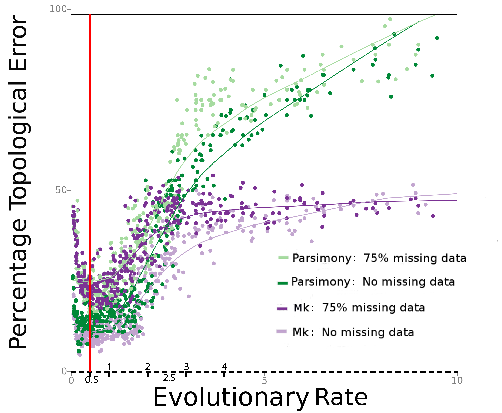
\includegraphics[keepaspectratio=true]{response_fig1.pdf}
\caption{Figure 3 from Wright and Hillis 2014 with added x axis ticks. The red line represents the 0.5 rate.}
\end{figure}

We do agree, however, that if rates get lower than 0.5, variance in topological error increases (especially for the Mk model with missing data).
Therefore, we implemented the \textit{a posteriori} matrix selection step to our analysis (i.e. keeping only the ``complete'' matrices that led to trees with a median bootstrap $>$ 50; explained lines 259-268 in the submitted manuscript and lines @@@ and @@@ in the revised one).

We rephrased the section highlighted by the reviewer as follows:

"We used low evolutionary rate parameters to be consistent with the molecular rate parameters, to avoid homoplasy in the morphological part of the matrix and create a clear phylogenetic signal (Wright and Hillis, 2014).
Topological error has been shown to be minimal at a morphological rate of 0.5 when using the M\textit{kv} model (Lewis, 2001; Wright and Hillis, 2014).
Note, however, that Wright and Hillis (2014) have shown that low morphological rates (< 0.5) increase variance in topological error, but we discarded simulations with such topological error by selecting only matrices with a “fair” phylogenetic signal (see Estimating phylogenies section below; Zander, 2004) so this should not influence our results." lines 211-217 @@@

% -----------------
% Specific Comment 23
% -----------------
\item{\textcolor{blue}{\textbf{line 201:} change 'get' for 'obtain' or something less colloquial.}}

We modified this whole section following reviewer 2 comment 2.

% -----------------
% Specific Comment 24
% -----------------
\item{\textcolor{blue}{\textbf{line 231-235:} streamline, e.g., 'The minimal dataset included in this study was 5\% of the morphological matrix for any taxon'.}}

We modified the sentence as follows: "To avoid avoid matrices containing taxa without any data (morphological or molecular), we repeated the random deletion until the matrices contained at least 5\% of data for any taxon." (line 264-267@@@).

% -----------------
% Specific Comment 25
% -----------------
\item{\textcolor{blue}{\textbf{line 237-246:} I understand the rational presented by the authors for comparing missing data trees to the best tree inferred from max. likelihood/Bayesian techniques rather than compare missing data trees to the true tree used to simulate the data. I still feel it would be an important contribution to this paper, however, to compare the missing data trees to the true tree to evaluate the effects of missing data on the tree inference. Also it may lend insights to whether the parameter settings used in the simulations and in the analyses were adequate for generating datasets and inferring the true tree, or something close to it. }}

We dealt with this comment above (Reviewer 1, major comment 6) and below (Reviewer 2 comment 1).

% -----------------
% Specific Comment 26
% -----------------
\item{\textcolor{blue}{\textbf{line 249:} condense citations to one parenthetical statement, 'GTR model (Tavare, 1986, default setting in RAx…)'. Also watch for citations in parentheses inside of other parenthetical statements on line 250 and throughout the manuscript. }}

We fixed these issues throughout the manuscript.

% -----------------
% Specific Comment 27
% -----------------
\item{\textcolor{blue}{\textbf{line 251:} omit 'implemented'}}

We removed this word.

% -----------------
% Specific Comment 28
% -----------------
\item{\textcolor{blue}{\textbf{line 273:} 'Bayesian Inference'}}

We changed the title as suggested.

% -----------------
% Specific Comment 29
% -----------------
\item{\textcolor{blue}{\textbf{line 286:} Why was the true tree used as a starting tree? Earlier the authors argued that the true tree is almost never known, so using it here detracts from the generalizability of these results. If the only justification is 'to speed up the Bayesian estimation process' as stated later, then it seems like this may bias one of the main results, which is that Bayesian analyses outperformed max. likelihood, in which no starting tree was used. I understand the computational limitations, but the authors should present some analysis with complete and missing data in which no starting tree is given compared to analyses in which a starting tree is given to evaluate whether using a starting tree significantly affects the resulting trees, perhaps in an Appendix. Or at least include some perturbation to the starting tree to avoid overly influencing the resulting topology. It would seem to me that this is illustrated in figure 5, where-in with the Robinson-Foulds metric, the distance to the best tree in Bayesian analysis seems to have a lower bound at ~0.7, even under the worst cases of missing data. This may be the worst the analysis can do given that it started out with the true tree. }}

We dealt with this comment above (see Reviewer 1 major comment 7).

% -----------------
% Specific Comment 30
% -----------------
\item{\textcolor{blue}{\textbf{line 318:} replace 'the twice number' with 'twice the number'}}

We fixed this typo.

% -----------------
% Specific Comment 31
% -----------------
\item{\textcolor{blue}{\textbf{line 327:} 'This methods' omit 's'}}

We fixed this typo.

% -----------------
% Specific Comment 32
% -----------------
\item{\textcolor{blue}{\textbf{line 343:} 'this metric is sensitive' add 'is'}}

We fixed this typo.

% -----------------
% Specific Comment 33
% -----------------
\item{\textcolor{blue}{\textbf{line 424:} 'Figure ??' should be Figure 6, but then do not repeat Figure 6 in the parentheses. }}

We fixed this typo.

% -----------------
% Specific Comment 34
% -----------------
\item{\textcolor{blue}{\textbf{line 436:} 'effect'}}

We fixed this typo as well as in the following sentence (line @@@).

% -----------------
% Specific Comment 35
% -----------------
\item{\textcolor{blue}{\textbf{line 489:} Streamline to something like: '…when the fossil is present near the tips but affects the clade conservation less when fossils are near the root'. }}

We modified the sentence as suggested.

% -----------------
% Specific Comment 36
% -----------------
\item{\textcolor{blue}{\textbf{line 494:} 'taxon'}}

We fixed this typo.

% -----------------
% Specific Comment 37
% -----------------
\item{\textcolor{blue}{\textbf{line 515:} '…the size of the matrix' missing 'of'}}

We fixed this typo.

% -----------------
% Specific Comment 38
% -----------------
\item{\textcolor{blue}{\textbf{line 518 to 520:} I am not sure that (Wagner 2000) states that incongruence between molecular and morphological data is 'more important in small morphological matrices'. }}

We now refer to two more classical citations: Bremer and Struwe 1992 (American Journal of Botany) and Patterson et al. 1993 (Annual Review of Ecology and Systematics), on phylogenetic signal and congruence between morphological and molecular data and also refer to a classical example of conflict probably due to having a small matrix (Masters and Brothers 2002; American Journal of Physical Anthropology; 36 characters) lines 578-579@@@.

% -----------------
% Specific Comment 39
% -----------------
\item{\textcolor{blue}{\textbf{line 520:} Either change 'size' to plural or change 'were' to 'was', the former seems to flow better. }}

We modified the sentence as follows: "The sizes of our data matrices were constrained by the performance of our protocol" (line 579-580@@@).

% -----------------
% Specific Comment 40
% -----------------
\item{\textcolor{blue}{\textbf{line 528:} missing close parenthesis after Ni et al.}}

We fixed this typo.

% -----------------
% Specific Comment 41
% -----------------
\item{\textcolor{blue}{\textbf{line 532:} Wright and Hillis 2014 found that increasing the size of the dataset improves topological accuracy, and they do not argue that simply increasing the number of characters increases the amount of homoplasy. Rather they found that the fastest evolving characters exhibited homoplasy, while the slowest evolving lacked phylogenetic signal. The citation seems misrepresented. Further, there was higher phylogenetic accuracy of simulated datasets with more characters than fewer characters, for slow or fast evolving characters (Wiens 2005).}}

We removed the entire statement concerning homoplasy and matrix size ("Homoplasy, on the other hand, is expected to increase with an increase in the number of morphological characters (Wright and Hillis 2014).")

% -----------------
% Specific Comment 42
% -----------------
\item{\textcolor{blue}{\textbf{line 540:} replace 'a lot' with 'larger proportions of missing data', a lot seems too colloquial for this kind of article. }}

We modified the sentence as suggested.

% -----------------
% Specific Comment 43
% -----------------
\item{\textcolor{blue}{\textbf{lines 542-547:} These seem like the most important practical results and should be more strongly emphasized. These are very important results for practitioners and the authors should try to make it more clear to the reader that this is a key take-home message.}}

We modified the paragraph to:

"Surprisingly, the number of missing living taxa with morphological data ($M_{L}$) and the overall number of missing morphological characters ($N_{C}$), have a bigger effect than the amount of missing data for the fossil taxa ($M_{F}$).
For any additional missing living taxa with morphological data ($M_L$) beyond 50\%, there is no difference among trees with any combination of the other parameters ($M_F$ and $N_C$; Figure 6).
In other words, when the number of missing living taxa reaches 50\%, neither the amount of missing data in the fossil record ($M_F$), nor the number of characters in the matrix ($N_C$) affect topology.
A similar effect can be observed when the $N_C$ parameter reaches 50 characters (Figure 6).
This has important practical implications, especially for the best strategy to improve topology by collecting more morphological data (see below)." lines 589-609@@@

% -----------------
% Specific Comment 44
% -----------------
\item{\textcolor{blue}{\textbf{line 552:} replace 'cladistic' with 'parsimony'. While one has come to be associated with the other in the literature, they are not synonymous. }}

We replaced 'cladistic' by 'parsimony' as suggested.

% -----------------
% Specific Comment 45
% -----------------
\item{\textcolor{blue}{\textbf{line 557-558:} '…than the "best" maximum likelihood tree'}}

We modified the sentence as suggested.

% -----------------
% Specific Comment 46
% -----------------
\item{\textcolor{blue}{\textbf{line 549-565:} again, I am left wondering how much the differences in performance of max. likelihood and Bayesian inference techniques are driven by the use of the 'true' tree as a starting tree in the Bayesian MCMC search, while the likelihood analysis had no such guide tree to begin with. The authors at least need to make this point clear, if not re-run some subset of analyses without introducing a starting tree to test the effects of using the 'true' tree as a starting tree or not. I understand the computational limitations, but the practical limitation that empiricists will never have the 'true' tree to start with may (or may not) have a large impact on our interpretation and the generality of these findings. }}

As discussed above (reviewer 1, specific comment 29), we understand the reviewer's concern and have added an analysis in Appendix A (figure A2 and tables A1 and A2) where we tested the effect of using the ``true'' tree as a starting tree. We found that there is no significant effect of using the ``true'' tree instead of a random tree (MrBayes default) as a starting tree on topological recovery.

We refer to this supplementary analysis in the main text as follows:

"Our results show that the topology of the Bayesian consensus tree is always closer to the ``best'' tree topology than the ``best'' Maximum Likelihood tree (Figure 5).
Note that the methodological choice of using the ``true'' tree as a starting tree for the Bayesian Inference rather than a random starting tree (see Methods), had no significant effect on topological recovery (see Appendix A, section ``Effect of the starting tree on Bayesian inference'' for details on the analysis of the effect of the starting tree in Bayesian inference)." lines 618-624@@@

% -----------------
% Specific Comment 47
% -----------------
\item{\textcolor{blue}{\textbf{line 593:} 'MorphoBank' - the 'b' should be capitalized in keeping with the authors' usage (O'Leary and Kaufman 2011)}}

We fixed this typo.

% -----------------
% Specific Comment 48
% -----------------
\item{\textcolor{blue}{\textbf{line 599:} remove extra close parenthesis inside parenthetical statement}}

We fixed this typo.

% -----------------
% Specific Comment 49
% -----------------
\item{\textcolor{blue}{\textbf{line 595-606:} this paragraph seems unsatisfactory advice for practitioners.
First, advising that the tree topology be fixed using the Bayesian consensus tree before conducting analyses such as dating strongly conditions the results on only a single tree and as the authors point out in the parenthetical statement, the dating information could improve accuracy. Indeed one of the many advantages of tip-dating is the joint inference of tree topology and divergence times.
The following statements that the posterior distribution should not be discarded does not leave the reader with a clear path that they should follow - if only the fixed tree topology is used to estimate divergence times, how can the substitution rate-scaled posterior distribution of highly probable trees be used for most comparative analyses which require time-scaled branch lengths?
This paragraph requires further justification and this study does have important bearing on a subject that gets little attention. }}

We revised the paragraph as follows:
"Another practical implication of our results regards the tree inference methods.
Because the Bayesian consensus trees consistently recovered topologies closer to the ``best'' tree topology than the Maximum Likelihood trees, we advise that where a topological constraint is needed, Bayesian consensus trees should be used. This may apply to tree inferences using the Total Evidence method such as tip-dating (e.g. Ronquist et al., 2012a; Wood et al., 2013; Matzke, 2014). It is, however, possible that including dating information during tree inference could also improve the accuracy of the Bayesian posterior tree distribution, so a fixed topology should be used with caution.
Using the Bayesian consensus tree rather than the Maximum Likelihood can also reduce the number of false positive topologies (Swofford et al., 2001).
As shown in figure 5 and discussed in the section above (Effects of tree inference methods), the Bayesian consensus tree is more likely to not resolve poorly supported nodes due to missing data than the Maximum Likelihood tree that is more likely to incorrectly resolve such nodes (i.e. creating a false positive node).
Note, however, that we do not suggest discarding the Bayesian posterior tree distributions even though they performed poorly in recovering the ``best'' tree topology in our simulations (this can probably be imputed to the difficulties comparing distributions of trees; see above).
These trees will be invaluable for phylogenetic comparative analyses. For example a sub-sample of posterior trees distributions can be used to assess macroecological questions while better taking into account topological uncertainty (e.g. Fritz et al. 2009 and Jetz et al. 2012 trees used in Healy et al. 2014)." lines 680-700@@@

% -----------------
% Specific Comment 50
% -----------------
\item{\textcolor{blue}{\textbf{line 612-613:} too obvious and not especially helpful. We should aim to have as little missing data as possible…more helpful, and something especially discovered in this study, is concentrating on having overlapping morphological characters between the living and fossil taxa to be able to place the living taxa with strong support via large datasets (combined data) and being able to position the fossils based on their shared derived characters with living taxa. This is an important point to make clearer. }}

Agreed. See reviewer 1 comment 11 for the changes to the conclusion.

% -----------------
% Specific Comment 51
% -----------------
\item{\textcolor{blue}{\textbf{line 613-615:} rephrase - sentence is choppy with all the commas. }}

We removed this sentence and replaced it by the two new sentences outlined above (reviewer 1 comment 11).

% -----------------
% Specific Comment 52
% -----------------
\item{\textcolor{blue}{\textbf{line 615-618:} It seems more important to me that the authors emphasize what implications it may have for previous and future studies that Bayesian analyses outperform max. likelihood, other than to re-hash that the authors feel the Bayesian consensus should be used to fix topologies for other downstream analyses.
For example, can the authors cite some combined analyses that used only likelihood analyses and came up with controversial results?
Or what about other studies that have done combined analyses with different optimality criteria and found different topologies?
What about implications for studies that have used molecular scaffold techniques to fix the topology of living taxa based on analyses of only DNA analyses and then fit the fossils into this fixed tree?
Also 'further' is misspelled.  }}

Unfortunately, we did not find many studies formally testing the important questions asked by the reviewer. However, there are a few empirical analyses that contain results supporting our claims.
Firstly, for the question about the topological differences between Maximum Likelihood and the Bayesian consensus tree, in Arcila et al 2015 (MPE)'s supplementary analysis, the authors compare the topology inferred from a Total Evidence matrix in both Likelihood (RAxML) and Bayesian (MrBayes) and the topology of the Bayesian consensus tree is much better supported than the one of the best ML tree. Specifically, the ML tree has 7/28 nodes have a "fair" bootstrap support ($>$ 75) and 3/28 with a good support ($>$ 90) as the Bayesian consensus tree has 17/25 nodes with a "fair" posterior probability ($>$80) and 14/25 with a good posterior probability ($>$95). We therefore used this reference to strengthen our claim of the superiority of the Bayesian consensus tree over the Maximum Likelihood one.

Secondly, for the question about molecular scaffolds, from the few studies clearly specifying their topological constraint method, only Beck and Lee 2013 (Proceedings B) seems to compare an analysis with and without taxonomic constraint on divergence time and rate estimation (the constraint seems to have no effect) but the branch length aspect is not covered in our study.

See our response to reviewer 1's comment 11 above for changes in the revised manuscript.

% -----------------
% Specific Comment 53
% -----------------
\item{\textcolor{blue}{\textbf{line 628:} use of computer cluster may be better placed in the methods, depending on the norm for MPE.}}

The Lonsdale cluster requires this specific line in the acknowledgements of any study using its infrastructure (\url{http://www.tchpc.tcd.ie/resources/acknowledgementpolicy}).
If requested, however, we can also give additional details on the cluster used in the methods section.
The current version of the manuscript only contains information on the nodes clock speed (2.30GHz clock speed nodes) lines @@@.

% -----------------
% Specific Comment 54
% -----------------
\item{\textcolor{blue}{\textbf{Figure 3:} Do not repeat the aside to similarity with t-test again from Fig 2 and text.}}

We removed the sentence about the t-test similarity from both figure captions.

% -----------------
% Specific Comment 55
% -----------------
\item{\textcolor{blue}{\textbf{Figure 4:} color codes in legend do not match up to the colors in the PDF I received. I don't know if this is an error in conversion, but the colors are black, red, green and blue in my PDF. The legend states the following: 'Maximum Likelihood trees (black), Bayesian consensus trees (blue), Maximum Likelihood bootstrap trees (orange) and Bayesian posterior tree distributions (blue)' which doesn't seem correct since blue is repeated. This makes interpreting the figure difficult for me at this time, but I assume given the text in the Results that the Bayesian methods are black and red in the figure I received, indicating they were closer to the best tree than max likelihood trees. Red and green should not be used together.}}

We apologies again for this silly mistake. We dealt with this comment above (see reviewer 1's comment 12).

% -----------------
% Specific Comment 56
% -----------------
\item{\textcolor{blue}{\textbf{Figure 5:} This figure best summarizes the results, and a version of this should be the Graphical Abstract, with legends for the color cods and spelling out the missing data parameters, and the Y axis could just be 'clade similarity index' or 'rouge taxon index' so that the reader doesn't need to know what the names of the metrics are to grasp the graphic.
But concerning the Normalized Triplets metric, according to the text and appendix, if this index is 0, the similarity of the missing data tree to the best tree is no more than random, and < 0 it is more different than random.
For the Bayesian analyses, many results had values < 0 but the axis is set to 0.
Why not illustrate the distribution of values that is < 0? %Fixed
From this result, it appears the Bayesian analysis does quite poorly with missing data in terms of rouge taxa, and worse than max. likelihood.
This figure also suggests to me that the methods perform pretty badly with missing data, in contrast to previous findings that missing data are not overly deleterious.
For example, when all data are complete except Mf=50\%, the normalized RF metric is <0.8.
Missing data for up to 50\% of characters has been suggested to still have high accuracy in uncovering the true tree (Wiens 2003; Wiens 2005), although for small datasets such as the one used in this study, the results show a similar decline in accuracy.
This is a point that should be expanded upon in the discussion - how these results compare to other missing data studies and what do they tell us about the performance of the inference methods with missing data?}}

We thank the reviewer for this excellent suggestion and modified our graphical abstract. We also fixed the Normalised Triplets metrics axis to range from -0.5 to 1. We added a horizontal dotted line at Triplets = 0 to make sure the reader notes this change of scale.

We also linked these results to previous studies (Wiens 2003; Systematic Biology) and discussed the negative values of the Normalised Triplets metric in the reviewer 1 comment 10 (see above).

% -----------------
% Specific Comment 57
% -----------------
\item{\textcolor{blue}{\textbf{Figure 6:} I think this may be the most important figure because it is demonstrating the probability of overlap between the distributions of the best trees and the missing data trees.
It took me a long time to figure it out, however, and to figure out why the top of the triangle is all orange.
I would have expected something more like in Appendix C Figure C2 or Fig. C3.
At first I understood this to indicate high probability of overlap of the missing data trees which had the most missing data with the best tree.
But after re-reading the legend and methods several times, I am interpreting it as follows: the top of the triangle indicates a similarly poor fit of the distributions of missing data trees to the best tree under all parameter combinations once there is a high proportion of missing data.
The point is raised in the Results that once missing data in the living portion is > 50\% then they all perform poorly, but it was not easy to grasp.
Somehow this figure needs to be spelled out better in the caption and results so the reader can grasp it more quickly and easily without having to go back to the methods section to completely figure out what is being represented.}}

We thank the reviewer for pointing out this difficulty and acknowledge that such graphical representations of so many pairwise comparisons might be confusing.
We have made the figure caption clearer, and the methods section explaining how we calculated this figure and the results.

We modified the figure caption as follows:
"The effects of missing data on topological recovery using Bayesian consensus trees. Both axes show the percentage of missing data from 0\% (white) to 75\% (black) for the three parameters: $M_{L}$ (upper line), $M_{F}$ (middle line) and $N_{C}$ (lower line). The topological recovery is measured as (A) the Normalised Robinson-Foulds metric and (B) the Normalised Triplets metric calculated using the Bhattacharyya Coefficient. The Bhattacharyya Coefficient values are indicated using a color gradient ranging from low probability of overlap in blue, to high probability of overlap in orange. Blue regions denote a poor overlap in Normalised metric values between the different parameter combinations (i.e. the parameters have a strong effect on the metric and thus the topological recovery). Conversely, orange regions denote a high overlap in Normalised metric values between the different parameter combinations (i.e. the parameters have a weak effect on the metric and thus the topological recovery)." 

We modified the methods section as follows:
"Because of the difficulties in representing so many pairwise comparisons in a meaningful way, we summarized these results as a heat map of Bhattacharyya Coefficients (see Figure 6).
In this type of figure, parameters that have similar effects on recovering the ``best'' topology (either positive or negative effects) will be denoted by similar colour patches in the heat map representation of these comparisons (see Figure 6)." lines 434-439@@@

We modified the results section as follows:
"Using both Normalised Robinson-Foulds and Normalised Triplets metrics from the Bayesian consensus trees, the parameter combination with no missing data (i.e. $M_{L}$ = 0\%, $M_{F}$ = 0\%, $N_{C}$ = 100) is always the most dissimilar to all the other parameter combinations (thin deep blue line at the base of Figure 6).
The Normalised Robinson-Foulds metric (median Bhattacharrya coefficient = 0.79; blue regions in Figure 6A), however, displays more dissimilarities than the Normalised Triplets metric (median Bhattacharrya coefficient = 0.81; blue regions in Figure 6B).
The orange upper triangle in Figure 6A shows a high probability of overlap of the Normalised Robinson-Foulds metric for the trees with the $M_{L}$ parameter $\geq$ 50\% (Figure 6A).
Once $M_{L}$ $\geq$ 50\%, there is no additional effect of $M_{F}$ and $N_{C}$, regardless of the amount of missing data in these parameters (Figure 6A).
Likewise, once $N_{C}$ $<$ 50, there is no additional effect of $M_{L}$ and $M_{F}$ as denoted by the high probability of Normalised Robinson-Foulds metric overlap (horizontal orange stripes between the blue regions Figure 6A).
In Figure 5 for the Normalised Robinson-Foulds metric, this can be interpreted as the overlap between the distributions once $M_L$=50\%." lines 480-497@@@

% -----------------
% Specific Comment 58
% -----------------
\item{\textcolor{blue}{\textbf{Table 1:} The wording of the caption is off - the second paragraph is awkward. 
Are these values the probabilities of overlap between the distributions of the 'best' tree versus trees from each inference method pooled across all combinations of missing data? That is what is described in methods line 397 but it doesn't say so in the caption.
Two things:\\
1)  Comparing to the tables in Appendix C, the distribution of probabilities of overlap between max. likelihood and Bayesian trees are higher in most missing data schemes in tables in the Appendices than the overall values given in Table 1. How could the max. likelihood and Bayesian trees be so different?\\
2)  Pooling across all missing data schemes seems to wash out the effect of tree-inference method. I am not sure what a better way to present these would be, but perhaps some kind of matrix where the cells are the joint probabilities of overlap of each method with each missing data category, and then the marginal probabilities would be the probabilities of overlap for each method, averaged over missing data categories, as well as the marginal probabilities of overlap for each missing data category, averaged across methods.  e.g, RF distance:\\
Missing data:   0   25  50      75      Marginal \\
BI              1   0.9 0.8     0.75    0.863 \\
ML              1   0.9 0.75    0.25    0.725 \\
Marginal        1   0.9 0.78    0.5     \\
This may not be feasible in the text due to space limitations, maybe tables like these could be added to an appendix.}}

We dealt with the caption of the Table 1 in reviewer 1 comment 14 above.

For the other two points:
1) We are not entirely sure if the reviewer means (i) why the two methods display such differences ; or (ii) why, within each method, the combination of parameters displays a difference between each single parameters ($M_LM_FM_C$ vs. $M_L$, $M_F$ and $M_C$).
In the first case, we think that the difference between the methods is due to the fact that the Maximum Likelihood trees are more likely to display ``false positive'' topologies (i.e. clades that are incorrect but can be well supported; or not) as the Bayesian consensus tree, when many data is missing, are more likely to collapse nodes, resulting in trees with less resolution but more ``conserved clades'' (i.e. the clade ((a;b);c)) could be collapsed in (a;b;c) which is still a corrected representation of the relations within the clades rather than ((b;c);a)).

In the second case, the fact that probabilities of overlap between the methods when the missing data parameters were taken separately (i.e. only the focal missing data parameter varies) was higher than the parameters combinations is probably just due to the overall amount of missing data.
In practice, when only one missing data parameter varies the two other parameters where set a 0\%, therefore resulting in matrices with a maximum of 75\%/2 missing data for $M_L$ and $M_F$ an 75\% maximum for $M_C$.
When combined, the maximum amount of missing data can be much higher, especially when each parameter is set a 75\% missing data, thus decreasing the probability of the ``missing-data'' trees to be similar to the ``best'' tree (see Table 1 in this response).

\begin{table}[!ht]
%\begin{adjustwidth}{-2.25in}{0in} % Comment out/remove adjustwidth environment if table fits in text column.
\caption{Distribution overlap between Maximum Likelihood (ML) and Bayesian consensus tree (BI) across all missing data parameters combinations (pooled) and every single missing data parameter individually ($M_L$, $M_F$, $N_C$)}
\centering
\begin{tabular}{|l|c|c|c|c|c|c|c|}
  \hline
 Comparison &  Metric & Min. & 1st Qu. & Median & Mean & 3rd Qu. & Max. \\ 
  \hline
    ML \textit{vs.} BI (pooled) & $RF$ & \textbf{0.00} & \textbf{0.00} & 0.10 & 0.20 & 0.32 & \textbf{1.00} \\ 
    ML \textit{vs.} BI ($M_L$)  & $RF$ & 0.30          & 0.31          & 0.69 & 0.61 & 0.77 & \textbf{1.00} \\ 
    ML \textit{vs.} BI ($M_F$)  & $RF$ & \textbf{0.00} & 0.25          & 0.48 & 0.50 & 0.76 & \textbf{1.00} \\ 
    ML \textit{vs.} BI ($N_C$)  & $RF$ & \textbf{0.03} & 0.32          & 0.66 & 0.55 & 0.75 & \textbf{1.00} \\
    ML \textit{vs.} BI (pooled) & $Tr$ & 0.34          & 0.49          & 0.61 & 0.62 & 0.75 & \textbf{1.00} \\
    ML \textit{vs.} BI ($M_L$)  & $Tr$ & 0.79          & 0.81          & 0.84 & 0.86 & 0.85 & \textbf{1.00} \\  
    ML \textit{vs.} BI ($N_C$)  & $Tr$ & 0.51          & 0.69          & 0.80 & 0.76 & 0.80 & \textbf{1.00} \\
    ML \textit{vs.} BI ($M_F$)  & $Tr$ & 0.38          & 0.69          & 0.75 & 0.72 & 0.80 & \textbf{1.00} \\  
   \hline
\end{tabular}
\label{Tab_Results-Difference_methods}
%\end{adjustwidth}
\end{table}


2) We followed the reviewer's suggestion and added six extra tables to Appendix C (Table C8 to C13) containing the marginal probability of each missing data parameter individually and for each tree inference method.

% -----------------
% Specific Comment 59
% -----------------
\item{\textcolor{blue}{\textbf{Appendix C:} Tables 1-3 repeats 'of the'. Should label the first two rows as 'Best maximum likelihood tree' and 'Best Bayesian inference tree'}}

We removed the repetition in the caption and changed the first two rows as suggested.
%If we understood the second point correctly, the reviewer suggests we add ``\textit{best}'' to the two first rows of the tables, and by ``\textit{best}'', the reviewer means ``optimal'' (as opposed to the ``best'' tree in our protocol that refers to any tree inferred by any method from the ``complete matrix''.
% We don't think it is necessary to follow this suggestion as the Maximum Likelihood tree is by definition the tree with the highest likelihood, and the Bayesian consensus is the consensus tree of the Bayesian inference trees.
%So adding the word ``\textit{best}'' here is not entirely accurate.

% NC: No we discussed this last night - I think they *do* mean "best" as in our protocol. So just make the changes to the first two rows.

% -----------------
% Specific Comment 60
% -----------------
\item{\textcolor{blue}{\textbf{Appendix D:} I find the online code repository thorough, but the repository is loaded with many files, especially for graphing. If it is possible to condense these files it may be easier for a reader to duplicate the study.}}

We updated the README page of the GitHub repository linking to the various R code to make it clearer what files are needed.
We also now provide a version of the analysis in R run throughout the manuscript as a step by step tutorial for a subset of data.
See \url{https://github.com/TGuillerme/Total_Evidence_Method-Missing_data/blob/master/Analysis/Analysis_Demo.R} and Appendix D.
We will also clean up this repository once the paper has been accepted.
At present it is functioning both as our working repository for code as well as the repository for this paper.

\end{enumerate}

\section{Reviewer 2:}
Note that we split the second comment from reviewer 2 in three different comments (comments 2,3 and 4 below) to improve the readability of our response to the reviewers.

% -----------------
% Comment 1
% -----------------
\begin{enumerate}
\item{\textcolor{blue}{\textbf{Compare the trees to the "true" tree:} I don't see how the "best" tree approach is helpful in this case. It adds an additional layer of complexity that can't be accounted for via simulation. The point of simulations is to compare empirical realities to the generating process, to see how much results diverge. I think the most helpful and straightforward thing to do is eliminate the "best" tree part of the MS, and compare the inferred trees directly to the real topology to quantify variance.}}

A similar point/suggestion was also raised by reviewer 1 and we ran the suggested extra analysis. See reviewer 1 general comment number 6 and specific comment number 25 for a detailed response.

We understand the concerns of the reviewer but, we would prefer to stick with our "best" tree approach.
In practice, the ``true'' tree can be perceived as a ``random'' seed to generate the ``complete'' matrix, as it simply a birth-death tree with $\lambda$ $>$ $\mu$ and a set number of living and fossil taxa (see details in the manuscript section "2.1 Generating the matrix").
All these parameters were only used to create a realistic ``complete'' matrix in order to make our results relevant to biologists. 

% NC: Can you rephrase a little here so it sounds less like you saying "no, and you're stupid". Doesn't the response to reviewer 1 cover this already? I've had a go but you may need to check what I've written.


% -----------------
% Comment 2
% -----------------
\item{\textcolor{blue}{\textbf{Better explanation of the missing data:} I found the explanation of the missing data strategy very difficult to follow. First, they oddly use the verb "to infer" for matrices; are they inferring matrices? Second, it's not clear anywhere that the authors actually removed the molecular data from the fossil taxa, though I assume they did. I hope the authors can re-write in simpler language ("explain like I'm 5") for easier comprehension.}}

The lines 180 and 181 states "All the molecular information for fossil taxa was replaced by missing data ("?")" in the former manuscript. We changed the verb "infer" (see specific comment number 16 from reviewer 1).

We assume the reviewer is referring to section "2.2 Removing data". We therefore modified the whole section to improve its clarity and simplicity as follows:

"To explore the effect of missing morphological data on topological recovery, we removed various amounts of the ``complete'' matrix to obtain matrices with missing morphological data.
Hereafter, we call these matrices with missing morphological data the ``missing-data'' matrices.
Note that the amount of molecular data remained constant throughout our simulations: 1000 molecular characters for living taxa and no molecular data for fossil taxa (see above).
We removed morphological data using three data incompleteness parameters:
\begin{enumerate}
\item{The proportion of missing living taxa ($M_L$).} This first missing-data parameter corresponds to the proportion of living taxa with no morphological data. It represents the number of living taxa that are present in the matrix but have only molecular data available. This reflects the fact that, because of the increasing ease of collecting molecular data, morphological data for living species is rarely collected (Guillerme and Cooper, 2015). Therefore, many living species will have only molecular data available. In practice, we removed all the morphological data from randomly chosen living taxa with five different proportions: 0\%, 10\%, 25\%, 50\% or 75\% of living taxa with no morphological data.
\item{The proportion of missing data in the fossil record ($M_F$).} This missing data parameter represents the completeness of the fossil record. Due to preservation biases, missing data for fossil taxa are common (Sansom and Wills, 2013). In practice, we randomly removed a proportion of data among the fossil taxa with five different proportions: 0\%, 10\%, 25\%, 50\% or 75\% of overall missing data for the fossil taxa.
%Added this part following comment 4.
Note that 50\% missing data for fossil taxa does not mean that each fossil is missing 50\% of its morphological data.
Instead this 50\% refers to missing fossil data across the whole matrix.
Some fossils may retain 100\% of their data and others may lose all their data at this parameter value (up to a maximum of 95\% missing data, see below). % NC: normally you'd say up to a maximum rather than up to a minimum. Is what I've written correct?
\item{The number of morphological characters for both living and fossil taxa ($N_C$).} This parameter is not a missing data parameter \textit{per se} but rather an indication of the size of the matrix. Any morphological matrix of any size has indeterminate missing data, given that the total number of characters is undefined, but presumably large. Therefore, this parameter corresponds to the overall number of characters available for both living and fossil taxa. In practice, we randomly removed whole characters from the morphological matrix reducing it to: 100, 90,75, 50 or 25 characters.
Note that these levels are equivalent to the two other parameters (i.e. 0\%, 10\%, 25\%, 50\% or 75\% of ``missing'' morphological characters).
\end{enumerate}

Each parameter represents a different way of removing data from the morphological part of the matrix: $M_L$ removes entire rows from the living data; $M_F$ removes cells from the fossil data; and $N_C$ removes columns across both living and fossil data. Note that $M_L$  and $M_F$ differ not only because of the region of the matrix affected: for $M_L$ all the morphological data of a percentage of living taxa are removed, whereas for $M_F$ a percentage of the data are removed at random from across the whole of the morphological matrix for fossil taxa.

We created matrices using all parameter combinations resulting in 125 ($5^3$) “missing-data” matrices. Note that one of these combinations ($M_L$=0\%; $M_F$=0\% and $N_C$=100) has no missing data so is equivalent to the “complete” matrix, thus we have one effectively complete matrix in our 125 “missing-data” matrices. In practice, we first removed the data following the two missing data parameters $M_L$ and $M_F$ and then removed data following the $N_C$ parameters. To avoid avoid matrices containing taxa without any data (morphological or molecular), we repeated the random deletion until the matrices contained at least 5\% of data for any taxon. Note that the living taxa always had at least 90\% of data (the 1000 molecular characters)." lines 222-267@@@


% -----------------
% Comment 3
% -----------------
\item{\textcolor{blue}{\textbf{$M_C$ is not missing data per se:} If Mc is just removing columns, then they are shrinking the total matrix. This is not missing data per se. They are instead comparing matrices of different sizes, and the quantity is "data present." Any matrix of any size has indeterminate missing data, given that the total number of characters is undefined, but presumably large. A matrix with 10,000 characters is tiny if 10,000,000 could be scored. This is semantic.}}

We agree with this comment and hope it will help to the global comprehension of the manuscript. We replaced the $M_C$ (missing characters) parameter by $N_C$ (number of characters with five states: 100, 90, 75, 50 and 25) in the revised manuscript (see reviewer 2 comment 2 above), the appendices and the figures. We also slightly modified some explanations related to the change of missing characters to number of characters throughout the manuscript.


% -----------------
% Comment 4
% -----------------
\item{\textcolor{blue}{\textbf{Specific variation of data per fossil:} More importantly, it doesn't seem like missing data varied among fossil taxa, unless I'm misreading. What we really want to know is what happens when some fossil taxa are fragmentary, as this is the most common empirical situation. Thus, there are morphological characters scored for some living taxa, some fossil taxa, and missing from others. It's unclear if this was simulated. It would be good if the authors could detail the case where, say, all living taxa had morphological data (0 Ml), the matrix was large (0 Mc), and Mf varied *among* fossil taxa, such that some fossils had 100\% coverage, and varied down to, say, 5\%. That's the crucial case here.}}

In this study, we applied a similar approach to what the reviewer 2 suggests (i.e. no missing data for living taxa, and maximal number of characters but various amount of missing data for the fossil taxa). 
These results are present in figure 4, central row.
However, we think we may have not explained ourselves entirely clearly. The amount of changes among the fossil taxa was not set to any specific amount of missing data per fossil (e.g. like the "artificial fossil" approach in Pattinson et al 2014, Syst. Biol.) but we rather treated the missing data in the "whole" fossil record.
Because our fossil taxa and their characters where randomly simulated, we didn't have any \textit{a priori} assumption on how to remove the data.
We therefore decided to randomly remove a certain amount of data among all the fossils.
For example, when removing 75\% of the data for the fossil taxa ($M_F$=75\%) different scenarios could happen, ranging from a "homogeneous" incompleteness data distribution (each specific fossil taxa had 75\% of missing data) to a "heterogeneous" incompleteness data distribution  (80\% of the specific fossil taxa had 5\% available data and 21\% of the specific fossil taxa had 100\% available data).
In empirical matrices, the incompleteness data distribution probably lies in between both models.

We added the following comment to the explanation on removing data (See our response to reviewer 2's comment 1).

Note that 50\% missing data for fossil taxa does not mean that each fossil is missing 50\% of its morphological data.
Instead this 50\% refers to missing fossil data across the whole matrix.
Some fossils may retain 100\% of their data and others may lose all their data at this parameter value (up to a maximum of 95\% missing data, see below).

\end{enumerate}

We hope we have responded to all these comments appropriately. Please let us know if you require any further information,\\
\bigskip

Thomas Guillerme (guillert@tcd.ie)\\
Natalie Cooper

\end{document}